\SourceLeaf{260}%
\noindent oder, da hier $\beta = b$ gesetzt werden muss,
\[
\tag*{7)} dfb = db\cdot\frac{\rho k}{\lambda} f(\rho-b),
\]

aus welcher Gleichung die Natur von $fb$ abgeleitet werden muss. Es wird durch Vertauschung [von $b$ mit $\rho-b$:]
\[
\tag*{8)} df(\rho-b) = -db\cdot\frac{\rho k}{\lambda} fb.
\]

Setzt man also
\[
f(\rho-b) + ifb = B,
\]
\[
f(\rho-b) - ifb = B',
\]
so wird
\[
dB = iB\cdot db\cdot\frac{\rho k}{\lambda}, \qquad dB' = -iB'\cdot db\cdot\frac{\rho k}{\lambda},
\]
also
\[
B = Ce^{ib\frac{\rho k}{\lambda}}, \qquad B' = C'e^{-ib\frac{\rho k}{\lambda}},
\]
wo $C, C'$ Constanten, welche sich aus der Bedingung bestimmen, dass für $b=0$ $B$ und $B'$ nach 5) [und weil $f0$ verschwindet] $=\frac{\lambda}{\rho}$ werden, also
\[
B = \frac{\lambda}{\rho} e^{ib\frac{\rho k}{\lambda}}, \qquad B' = \frac{\lambda}{\rho} e^{-ib\frac{\rho k}{\lambda}}.
\]

Es ist folglich
\[
fb = \frac{\lambda}{\rho}\sin\left(\frac{\rho k}{\lambda}\cdot b\right), \qquad f(\rho-b) = \frac{\lambda}{\rho}\cos\left(\frac{\rho k}{\lambda}\cdot b\right),
\]
[mithin für $b=\rho$ nach 5):]
\[
1 = \sin\frac{\rho\rho k}{\lambda},
\]
woraus
\[
\frac{\rho\rho k}{\lambda} = \tfrac{1}{2}\pi,
\]
also
\[
fb = \frac{\lambda}{\rho}\sin\left(\frac{\pi}{2\rho}\cdot b\right)
\]
\Needspace{29\baselineskip}
[folgt. Für unendlich kleine $a$ hat mithin das Viereck $ACBD$ den Flächeninhalt
\[
a\frac{\lambda}{\rho}\sin\left(\frac{\pi}{2\rho} b\right).]
\]

\begin{center}\begin{minipage}{\linewidth}\centering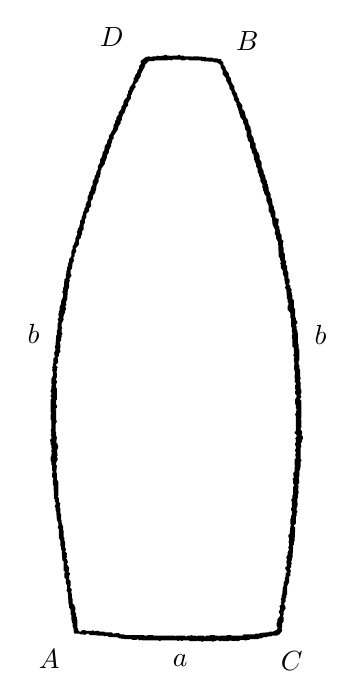
\begin{tikzpicture}[x=0.00870406cm,y=-0.00870406cm]
\fill[even odd rule] (198,82) -- (197,83) -- (195,83) -- (187,89) -- (188,93) -- (186,95) -- (185,97) -- (185,100) -- (183,102) -- (182,106) -- (179,110) -- (179,112) -- (177,114) -- (177,118) -- (176,119) -- (176,121) -- (171,128) -- (171,130) -- (169,133) -- (169,136) -- (167,139) -- (167,142) -- (164,145) -- (162,149) -- (162,152) -- (159,156) -- (159,159) -- (155,164) -- (155,167) -- (152,171) -- (152,174) -- (150,176) -- (150,179) -- (148,182) -- (147,189) -- (145,191) -- (144,194) -- (141,198) -- (141,202) -- (139,204) -- (138,209) -- (135,213) -- (134,220) -- (132,222) -- (131,228) -- (128,233) -- (128,237) -- (125,242) -- (125,247) -- (123,250) -- (122,255) -- (120,257) -- (120,260) -- (117,265) -- (117,270) -- (115,273) -- (114,278) -- (112,281) -- (112,283) -- (110,287) -- (110,293) -- (108,295) -- (108,297) -- (107,298) -- (107,302) -- (105,304) -- (105,307) -- (103,310) -- (103,313) -- (101,317) -- (101,320) -- (99,322) -- (99,327) -- (98,328) -- (98,331) -- (96,333) -- (95,337) -- (94,338) -- (95,341) -- (92,348) -- (92,352) -- (90,355) -- (90,357) -- (88,359) -- (88,363) -- (86,367) -- (86,374) -- (83,378) -- (83,381) -- (82,382) -- (82,384) -- (81,385) -- (81,389) -- (80,390) -- (80,394) -- (79,395) -- (79,399) -- (78,400) -- (78,406) -- (76,408) -- (75,419) -- (74,420) -- (74,424) -- (73,425) -- (73,427) -- (74,428) -- (74,433) -- (71,440) -- (71,444) -- (69,448) -- (69,453) -- (68,454) -- (68,457) -- (67,458) -- (68,463) -- (66,466) -- (67,468) -- (67,471) -- (66,472) -- (66,481) -- (65,482) -- (65,489) -- (64,490) -- (63,504) -- (62,505) -- (63,511) -- (61,515) -- (62,521) -- (60,523) -- (60,530) -- (59,531) -- (59,535) -- (58,536) -- (59,538) -- (58,540) -- (59,542) -- (59,549) -- (57,553) -- (57,560) -- (58,562) -- (57,563) -- (57,568) -- (56,569) -- (56,572) -- (57,573) -- (57,576) -- (56,577) -- (56,579) -- (57,580) -- (57,582) -- (56,583) -- (56,602) -- (57,603) -- (56,605) -- (56,613) -- (57,614) -- (57,626) -- (56,627) -- (57,633) -- (56,635) -- (57,636) -- (57,640) -- (55,642) -- (55,644) -- (56,645) -- (56,649) -- (57,650) -- (57,654) -- (58,655) -- (57,657) -- (57,660) -- (58,662) -- (57,663) -- (57,666) -- (56,667) -- (56,673) -- (57,674) -- (57,678) -- (58,679) -- (58,687) -- (59,688) -- (59,690) -- (58,691) -- (58,696) -- (60,699) -- (59,701) -- (59,707) -- (60,708) -- (61,728) -- (62,729) -- (62,732) -- (63,733) -- (63,737) -- (62,738) -- (62,740) -- (63,741) -- (63,745) -- (64,746) -- (65,759) -- (67,763) -- (67,768) -- (66,770) -- (68,773) -- (68,785) -- (70,789) -- (70,797) -- (71,798) -- (71,802) -- (72,803) -- (73,818) -- (75,820) -- (75,833) -- (77,835) -- (76,837) -- (76,843) -- (78,845) -- (78,851) -- (80,855) -- (80,860) -- (79,862) -- (81,865) -- (82,882) -- (83,883) -- (83,887) -- (85,890) -- (85,897) -- (86,898) -- (86,905) -- (87,906) -- (87,909) -- (88,910) -- (88,915) -- (89,916) -- (90,924) -- (91,925) -- (98,925) -- (99,926) -- (104,926) -- (105,927) -- (109,925) -- (111,925) -- (113,927) -- (123,927) -- (124,928) -- (133,928) -- (134,929) -- (139,928) -- (141,930) -- (153,930) -- (156,932) -- (159,932) -- (160,933) -- (162,932) -- (164,933) -- (174,933) -- (175,934) -- (181,934) -- (183,933) -- (186,935) -- (188,934) -- (190,935) -- (214,935) -- (215,936) -- (217,935) -- (241,935) -- (242,936) -- (244,935) -- (246,935) -- (247,936) -- (249,935) -- (258,935) -- (259,936) -- (269,936) -- (271,935) -- (272,936) -- (276,936) -- (277,937) -- (279,936) -- (291,936) -- (293,937) -- (294,936) -- (297,936) -- (298,935) -- (301,935) -- (302,936) -- (305,936) -- (306,935) -- (308,936) -- (316,936) -- (317,935) -- (325,936) -- (327,935) -- (328,936) -- (330,936) -- (334,934) -- (342,935) -- (343,934) -- (346,934) -- (347,933) -- (359,933) -- (360,932) -- (363,932) -- (367,930) -- (372,930) -- (373,929) -- (378,929) -- (379,928) -- (386,928) -- (390,926) -- (394,921) -- (393,917) -- (394,916) -- (394,910) -- (396,907) -- (396,901) -- (395,899) -- (396,898) -- (396,893) -- (399,888) -- (398,884) -- (397,883) -- (397,880) -- (399,878) -- (399,873) -- (400,872) -- (400,869) -- (401,868) -- (401,856) -- (404,850) -- (404,842) -- (406,840) -- (406,835) -- (407,834) -- (405,830) -- (407,828) -- (407,824) -- (408,823) -- (407,819) -- (408,818) -- (408,815) -- (409,814) -- (410,796) -- (411,795) -- (411,791) -- (412,790) -- (413,770) -- (411,768) -- (411,767) -- (414,764) -- (414,754) -- (415,753) -- (415,749) -- (416,748) -- (416,746) -- (415,745) -- (415,741) -- (416,740) -- (416,737) -- (417,736) -- (416,734) -- (416,728) -- (417,727) -- (417,721) -- (418,720) -- (418,717) -- (417,716) -- (418,710) -- (417,708) -- (419,704) -- (418,697) -- (419,696) -- (419,687) -- (420,686) -- (420,683) -- (421,682) -- (421,674) -- (422,673) -- (422,671) -- (421,670) -- (421,653) -- (422,652) -- (421,647) -- (423,645) -- (423,642) -- (424,641) -- (424,637) -- (422,635) -- (423,633) -- (423,630) -- (421,627) -- (421,625) -- (422,624) -- (422,613) -- (421,612) -- (422,610) -- (422,585) -- (420,583) -- (420,582) -- (422,579) -- (421,577) -- (421,575) -- (422,574) -- (422,569) -- (421,568) -- (421,558) -- (420,557) -- (420,554) -- (421,553) -- (421,551) -- (420,550) -- (420,539) -- (419,538) -- (419,533) -- (418,532) -- (418,527) -- (419,526) -- (419,510) -- (418,509) -- (418,502) -- (417,501) -- (417,486) -- (416,485) -- (416,482) -- (415,481) -- (415,476) -- (414,475) -- (414,474) -- (416,472) -- (416,469) -- (414,467) -- (414,464) -- (413,463) -- (413,451) -- (411,449) -- (411,438) -- (409,436) -- (409,431) -- (408,430) -- (408,427) -- (407,426) -- (408,423) -- (406,420) -- (406,417) -- (404,415) -- (404,413) -- (405,412) -- (405,408) -- (403,406) -- (403,398) -- (401,394) -- (401,388) -- (399,386) -- (400,382) -- (398,379) -- (398,371) -- (396,368) -- (396,361) -- (395,360) -- (395,354) -- (396,352) -- (393,349) -- (393,343) -- (391,340) -- (391,336) -- (390,335) -- (390,332) -- (388,328) -- (389,320) -- (388,319) -- (386,319) -- (384,317) -- (384,309) -- (382,305) -- (382,302) -- (380,299) -- (379,290) -- (377,288) -- (377,283) -- (374,277) -- (374,273) -- (373,272) -- (373,269) -- (372,268) -- (372,264) -- (370,262) -- (369,256) -- (367,253) -- (367,250) -- (364,244) -- (364,237) -- (361,232) -- (361,227) -- (360,226) -- (360,224) -- (357,220) -- (357,218) -- (355,215) -- (355,209) -- (353,207) -- (352,201) -- (349,196) -- (349,190) -- (348,189) -- (348,186) -- (345,181) -- (344,175) -- (341,171) -- (339,162) -- (336,159) -- (336,154) -- (331,147) -- (331,144) -- (329,142) -- (328,136) -- (326,134) -- (324,130) -- (324,126) -- (320,120) -- (319,114) -- (316,110) -- (316,107) -- (312,102) -- (311,98) -- (308,94) -- (308,91) -- (305,88) -- (305,87) -- (304,86) -- (300,86) -- (299,85) -- (293,85) -- (292,84) -- (283,84) -- (282,83) -- (277,83) -- (276,82) -- (274,83) -- (272,82) -- (264,82) -- (262,83) -- (261,82) -- (251,82) -- (250,81) -- (245,81) -- (244,80) -- (242,80) -- (241,81) -- (233,81) -- (232,82) -- (230,81) -- (226,81) -- (225,80) -- (222,80) -- (221,81) -- (218,81) -- (217,82) -- (211,81) -- (210,82) -- (205,82) -- (204,83) -- cycle
(199,89) -- (207,89) -- (208,88) -- (226,88) -- (227,87) -- (233,88) -- (235,86) -- (237,87) -- (246,87) -- (247,88) -- (252,88) -- (253,87) -- (257,87) -- (258,88) -- (275,88) -- (276,89) -- (294,90) -- (295,91) -- (298,91) -- (302,93) -- (304,95) -- (304,98) -- (307,103) -- (307,108) -- (312,114) -- (312,117) -- (317,126) -- (317,129) -- (320,133) -- (320,135) -- (323,141) -- (324,146) -- (327,150) -- (327,153) -- (328,154) -- (328,156) -- (329,157) -- (333,171) -- (337,176) -- (337,179) -- (339,183) -- (340,189) -- (342,191) -- (342,199) -- (343,200) -- (344,205) -- (347,208) -- (347,215) -- (349,218) -- (350,223) -- (352,225) -- (353,233) -- (356,240) -- (356,243) -- (358,246) -- (358,251) -- (360,254) -- (360,256) -- (362,260) -- (362,264) -- (365,269) -- (365,274) -- (366,275) -- (366,278) -- (367,279) -- (368,283) -- (371,287) -- (371,293) -- (374,300) -- (374,308) -- (377,312) -- (377,315) -- (379,318) -- (380,328) -- (384,336) -- (383,341) -- (385,344) -- (385,348) -- (388,353) -- (389,375) -- (391,377) -- (391,380) -- (392,381) -- (392,383) -- (391,384) -- (392,386) -- (392,391) -- (395,395) -- (395,400) -- (397,404) -- (397,409) -- (398,410) -- (398,414) -- (399,415) -- (399,418) -- (398,420) -- (400,423) -- (401,436) -- (402,437) -- (402,441) -- (403,442) -- (403,445) -- (402,446) -- (402,452) -- (406,457) -- (406,464) -- (407,465) -- (407,477) -- (408,478) -- (408,485) -- (409,486) -- (409,488) -- (408,489) -- (408,494) -- (409,495) -- (409,506) -- (411,508) -- (411,517) -- (410,519) -- (412,521) -- (411,523) -- (411,528) -- (412,529) -- (411,539) -- (412,540) -- (412,543) -- (413,544) -- (413,546) -- (412,547) -- (412,552) -- (413,553) -- (412,557) -- (414,559) -- (414,561) -- (413,562) -- (413,568) -- (414,569) -- (413,571) -- (413,575) -- (415,577) -- (415,579) -- (413,583) -- (413,590) -- (414,591) -- (414,596) -- (415,597) -- (414,603) -- (413,604) -- (413,606) -- (414,607) -- (414,629) -- (412,631) -- (412,632) -- (415,635) -- (415,637) -- (413,640) -- (414,642) -- (414,646) -- (413,647) -- (413,650) -- (414,651) -- (414,655) -- (413,656) -- (413,659) -- (414,660) -- (414,662) -- (413,663) -- (414,669) -- (412,671) -- (412,679) -- (413,681) -- (412,682) -- (412,688) -- (410,691) -- (411,697) -- (409,699) -- (410,701) -- (410,706) -- (411,707) -- (411,710) -- (410,711) -- (410,722) -- (409,723) -- (409,727) -- (407,730) -- (408,732) -- (408,741) -- (407,742) -- (407,745) -- (408,746) -- (408,752) -- (407,753) -- (407,756) -- (406,757) -- (406,765) -- (407,767) -- (406,768) -- (405,779) -- (403,781) -- (403,784) -- (404,785) -- (404,790) -- (403,791) -- (404,793) -- (404,797) -- (403,798) -- (403,800) -- (404,802) -- (402,806) -- (402,810) -- (400,813) -- (400,815) -- (401,816) -- (401,818) -- (400,819) -- (401,826) -- (398,829) -- (401,835) -- (399,837) -- (399,842) -- (398,843) -- (398,847) -- (396,851) -- (396,856) -- (395,857) -- (394,868) -- (393,869) -- (393,873) -- (392,874) -- (392,876) -- (393,877) -- (392,880) -- (393,882) -- (390,885) -- (391,887) -- (391,890) -- (389,892) -- (389,894) -- (391,897) -- (391,899) -- (387,904) -- (387,908) -- (386,909) -- (386,914) -- (387,915) -- (387,918) -- (385,920) -- (381,922) -- (375,922) -- (374,923) -- (362,924) -- (361,925) -- (355,925) -- (354,926) -- (338,926) -- (336,928) -- (320,928) -- (319,927) -- (314,927) -- (313,928) -- (303,928) -- (301,929) -- (300,928) -- (296,928) -- (295,927) -- (289,927) -- (288,928) -- (283,928) -- (282,929) -- (280,929) -- (279,928) -- (271,928) -- (269,929) -- (268,928) -- (263,928) -- (261,927) -- (260,928) -- (256,928) -- (255,929) -- (253,929) -- (252,928) -- (240,928) -- (238,929) -- (237,928) -- (206,928) -- (205,927) -- (198,927) -- (197,928) -- (193,928) -- (192,927) -- (164,927) -- (163,926) -- (158,926) -- (155,924) -- (147,925) -- (145,923) -- (135,923) -- (134,922) -- (127,922) -- (126,921) -- (122,921) -- (120,922) -- (118,920) -- (116,921) -- (107,921) -- (106,920) -- (102,920) -- (100,922) -- (98,922) -- (96,920) -- (96,918) -- (95,917) -- (95,905) -- (94,904) -- (94,901) -- (93,900) -- (93,895) -- (91,893) -- (92,891) -- (92,887) -- (91,886) -- (91,884) -- (88,881) -- (88,874) -- (87,873) -- (87,867) -- (86,866) -- (86,863) -- (87,861) -- (84,857) -- (85,855) -- (85,848) -- (83,846) -- (83,840) -- (84,839) -- (84,837) -- (82,835) -- (83,829) -- (80,824) -- (80,822) -- (81,821) -- (80,817) -- (79,816) -- (79,814) -- (80,813) -- (79,810) -- (80,808) -- (77,805) -- (78,803) -- (78,801) -- (77,800) -- (77,791) -- (76,790) -- (76,785) -- (75,784) -- (75,775) -- (74,774) -- (74,768) -- (73,767) -- (73,765) -- (72,764) -- (72,760) -- (71,759) -- (71,750) -- (70,749) -- (70,742) -- (69,741) -- (70,735) -- (68,733) -- (68,727) -- (66,725) -- (67,723) -- (67,703) -- (65,700) -- (65,691) -- (64,690) -- (65,680) -- (64,679) -- (64,675) -- (66,671) -- (66,669) -- (65,668) -- (65,666) -- (66,665) -- (65,657) -- (66,656) -- (67,651) -- (66,650) -- (66,648) -- (64,646) -- (65,638) -- (64,637) -- (64,631) -- (63,630) -- (63,619) -- (65,615) -- (64,613) -- (64,599) -- (63,598) -- (63,597) -- (65,595) -- (65,592) -- (64,591) -- (64,584) -- (65,583) -- (65,567) -- (64,566) -- (64,560) -- (65,559) -- (65,556) -- (64,555) -- (64,552) -- (65,551) -- (65,545) -- (64,543) -- (65,542) -- (65,538) -- (66,537) -- (66,536) -- (64,534) -- (64,532) -- (67,529) -- (66,522) -- (68,519) -- (68,516) -- (70,514) -- (70,511) -- (69,510) -- (70,508) -- (70,502) -- (69,500) -- (71,497) -- (71,493) -- (72,492) -- (72,489) -- (73,488) -- (73,486) -- (72,485) -- (72,480) -- (73,479) -- (72,477) -- (72,472) -- (75,466) -- (74,463) -- (75,462) -- (75,460) -- (77,456) -- (77,453) -- (78,452) -- (78,449) -- (77,447) -- (79,445) -- (78,441) -- (80,437) -- (81,423) -- (83,419) -- (83,411) -- (84,410) -- (83,407) -- (86,403) -- (86,401) -- (85,400) -- (85,394) -- (87,392) -- (88,383) -- (90,381) -- (89,376) -- (91,374) -- (91,370) -- (93,368) -- (93,365) -- (92,363) -- (97,357) -- (97,350) -- (100,347) -- (100,345) -- (102,341) -- (102,337) -- (104,335) -- (104,328) -- (106,325) -- (106,320) -- (108,317) -- (108,312) -- (112,308) -- (112,304) -- (115,301) -- (115,298) -- (114,296) -- (115,295) -- (115,293) -- (117,291) -- (118,285) -- (121,281) -- (121,279) -- (122,278) -- (123,270) -- (126,265) -- (126,260) -- (128,258) -- (128,255) -- (129,254) -- (129,249) -- (130,248) -- (130,246) -- (135,239) -- (135,237) -- (138,230) -- (138,227) -- (141,222) -- (141,219) -- (144,213) -- (144,210) -- (145,209) -- (146,204) -- (148,202) -- (148,198) -- (154,189) -- (155,184) -- (158,180) -- (158,177) -- (160,175) -- (160,171) -- (161,170) -- (161,168) -- (164,164) -- (166,157) -- (169,154) -- (169,150) -- (171,146) -- (173,144) -- (173,139) -- (175,137) -- (175,135) -- (178,129) -- (180,127) -- (179,123) -- (184,118) -- (184,116) -- (187,112) -- (188,107) -- (193,98) -- (194,94) -- cycle;
\node[inner sep=0pt] at (145,54) {$D$};
\node[inner sep=0pt] at (343,59) {$B$};
\node[inner sep=0pt] at (31,488) {$b$};
\node[inner sep=0pt] at (450,489) {$b$};
\node[inner sep=0pt] at (54,962) {$A$};
\node[inner sep=0pt] at (408,965) {$C$};
\node[inner sep=0pt] at (245,965) {$a$};
\end{tikzpicture}
\\[3pt]Fig. 6.\end{minipage}\end{center}
